\documentclass{article}
\usepackage[utf8]{inputenc}
\usepackage{graphicx}
\usepackage{listings}
\usepackage{float}
\usepackage{indentfirst}
\usepackage{xcolor}
\usepackage{fmtcount}
\usepackage{geometry}
\usepackage{hyperref}
\geometry{margin=1in}

\lstset{basicstyle=\ttfamily\color{blue}}
\newcommand{\code}[1]{\lstinline|#1|}

\title{EEL 4712C - Digital Design: Lab Report 4}
\author{Cole Rottenberg \\ 11062528}
\date{March 3\textsuperscript{rd}, 2024}

\lstset{
  language=VHDL,
  numbers=left,
  stepnumber=1,
  tabsize=2,
  numbersep=5pt,
  backgroundcolor=\color{white},
  showspaces=false,
  showtabs=true,
  frame=single,
  rulecolor=\color{black},
  captionpos=b,
  breaklines=true,
  breakatwhitespace=true,
  title=\lstname,
}

\begin{document}

\maketitle

% Test VHDL code
% \begin{lstlisting}[caption=Test VHDL Code, label=lst:test-vhdl-code]
% -- This is a test VHDL code block
% library IEEE;
% use IEEE.STD_LOGIC_1164.ALL;
% use IEEE.STD_LOGIC_ARITH.ALL;

% entity test is
%     Port ( a : in  STD_LOGIC;
%            b : in  STD_LOGIC;
%            c : out  STD_LOGIC);
% end test;
% \end{lstlisting}

% \section*{Prelab Report}

% \subsection*{Prelab Questions}
% % Put all the answers to the prelab questions. These may be scanned using your phone or scanner. Not all prelabs have prelab questions

% \subsection*{Prelab Design and Implementation}
% % Go into detail about how you designed any design parts of the prelab. Then, go into detail about how you implemented any implementation parts of the prelab

% \subsection*{Reflection}
% % Talk about what you learned during the prelab. Bring up anything that was a stumped you for a while. Bring up any accomplishments you were proud of.

% \subsection*{Prelab Homework}
% % Show all work for the Prelab Homework here
% % Show all the work for every step in the Prelab Homework section. Label each part clearly and caption all figures. All simulations must be annotated. Annotation means pointing out particularly important parts of a simulation. This can be done with arrows or textboxes. Simple simulations will not have a lot to talk about, but later simulations will be a lot more complex. Any code written in the prelab should be commented a fair amount.

\section*{Lab Report}

\subsection*{Problem Statement}
% Provide a short informal description of the lab’s goals (From the lab assignment)
% If required, specify the system to design.
% - Define the inputs.
% - Define the outputs.
% - Define the function of your system. 
% This section should be 1-2 paragraphs long.
  The lab is broken into 4 individual parts and two groups of two. The first part deals with static timing analysis and the second part deals with implementing a basic VGA driver to display a box on a monitor. The third part deals with implementing a VGA driver to display a moving box on a monitor. The fourth part deals applying the same static timing analysis from the first part to the moving box from the third part.

  The 2\textsuperscript{nd} and 3\textsuperscript{rd} part of the lab are the critical design parts of the lab that help us explore the capabilities of the VGA driver and how to implement it. The first and fourth part are more about understanding the timing of the VGA driver and how to properly implement it. The part two is split into three different entities(primarily), the VGA, the VGA sync generator, and the top level component. The inputs to the top level component are relatively static and aren't changing. The outputs are the VGA signals that are sent to the monitor. The signals sent to the monitor are the h\_sync, v\_sync, and the RGB signals. The system is designed to display a box on the monitor. The sync generator is responsible for generating the sync signals, however the VGA entity is responsible for applying the logic to these signals to display the box on the monitor.

\subsection*{Design}
% Describe the design decisions you made.
% - What components did you use?
% - What signals did you use to connect the components?
% - What algorithms did you use?
% Code Segment or block diagrams may be included here.
% Explain your design choices(pros/cons).
% Any designs made in prelab should be included here but more briefly.
% This section should be 1-2 paragraphs long.

The VGA sync generator is consisted of a single clocked process that iterates through a double condition statement. The first conditionally block check if the \code{h_count} is equal the \code{H_MAX} constant defined in our package. If they are equal to eachother, we reset the counter and go onto the next conditional block, which checks if the \code{v_count} is equal to the \code{V_MAX} constant defined in our package. If they are equal to eachother, we reset the counter and exit the process. However, if we the first conditional is false, we increment the \code{h_count} counter. If the second conditional is false, we increment the \code{v_count} counter. On a conceptual level this builds a sweeping motion across the rows and then columns until the end. The second part of the generator exist outside a process as three conditions for the \code{h_sync}, \code{v_sync}, and \code{video_on} signals.

These signals are then passed up to the VGA entity which uses the \code{h_count} and \code{v_count} signals to determine the position of the box on the screen. The \code{draw} clocked process uses these counts to determine if the current pixel is within the define constants of: \code{CENTER\_X\_START}, \code{CENTER\_X\_END}, \code{CENTER\_Y\_START}, and \code{CENTER\_Y\_END}. If the pixel is within these bounds, the \code{red}, \code{green}, and \code{blue} signals are set to "0111", "0011", and "1011" respectively. Outside of the process, existing within the architecture, the \code{h_sync}, \code{v_sync}, and \code{video_on} signals are being outputted to the top level component.

The design of the 3\textsuperscript{rd} part builds of the previous part as it uses an identical VGA sync generator. The VGA entity is modified and new values are used to move the box across the screen as well as change the direction of the box. We also need to make use of a clock divider to slow down the clock signal to 1Hz. This \code{slow\_clk} signal is then used to drive our \code{obj\_move} process. This process is responsible for moving the box across the screen. The \code{obj\_move} process uses a new set of signals and constants to determine the position of the box on the screen. It also uses logic to control directional changes when the box reaches the vertical or horizontal bounds of the screen.

The top level entity controls the final output of the VGA signals to the monitor. The VGA entity passes the following outputs to the top level entity: \code{h\_sync}, \code{v\_sync}, \code{red}, \code{green}, \code{blue}, and \code{video\_on}. The top level entity then passes these signals to the VGA port which is connected to the monitor. 

\subsection*{Implementation}
% Describe the implementation process.
% Code segments or block diagrams may be included here.
% What time did you need to complete your design?
% This section should be 1-2 paragraphs long.
The implementation process was relatively straightforward with a "few" hiccups along the way. The first part of implementation was to implement the VGA sync generator. Knowing the defined input of specific clock signals left us to worry about the logic of iterating through the valid sections of the monitor. As seen in the code below, Listing \ref{lst:vga-sync-gen-part-2}, the process iterates through the horizontal and vertical counters. The second part of the implementation was to implement the VGA entity. This was a bit more complex as we had to determine the position of the box on the screen. However, given the constants defined in the package, we were able to easily determine the position of the box on the screen. In Listing \ref{lst:vga-entity-part-2}, we can see the logic used to determine the position of the box on the screen. Keep in mind some description comments were removed for brevity.

In 3\textsuperscript{rd} part of the lab, we had to implement a clock divider to slow down the clock signal to 1Hz. Considering we had already implemented a clock divider in a previous lab, we needed to change a few names of the IO and some generic logic for clock divider control. The implementation of the clock divider can be seen in Listing \ref{lst:clock-divider-part-3}. The implementation of the VGA entity was more comlex as we had to implement a new set of signals and constants to move the box across the screen. We also had to implement logic to control the direction of the box when it reached the bounds of the screen. The implementation of the VGA entity can be seen in Listing \ref{lst:vga-entity-part-3}.

\subsection*{Testing}
% Describe how you tested your design.
% Did everything work as expected?
% - Did inputs match the expected outputs?
% - Special cases?
% Include if possible, timing diagram of photo/video of the system.
There were multiple methods of testing the design and implementation. The 1\textsuperscript{st} method was to use the newly introduce timing analyzer tool in the Quartus Suite. This tool allowed use to check the timing of the VGA signals and ensure they were within the proper range. As seen in Figure \ref*{fig:timing-analysis}, by adjusting our clock capabilities to match our board's true clock period, we have ample time to display the box on the screen. The 2\textsuperscript{nd} method was to use the top level testbench.

\subsection*{Conclusions}
% Summarize in one paragraph, the work you did, the success and problems you encountered, and how to improve next in the future.
% This section should only be 1 paragraph long.

\section*{Appendix}
% Include all postlab code, screenshots, and simulations here. ALL SIMULATIONS MUST BE ANNOTATED. This means pointing out particularly important parts of a simulation. This can be done with arrows or textboxes. All figures must be captioned. Code should be commented a fair amount.

\begin{lstlisting}[caption=VGA Sync Generator for Part 2, label=lst:vga-sync-gen-part-2]
library ieee;
use ieee.std_logic_1164.all;
use ieee.numeric_std.all;
use work.VGA_LIB.all;

entity vga_sync_gen is
    port (
        clk       : in std_logic;
        rst       : in std_logic;
        h_count   : out std_logic_vector(COUNT_RANGE);
        v_count   : out std_logic_vector(COUNT_RANGE);
        h_sync    : out std_logic;
        v_sync    : out std_logic;
        video_on  : out std_logic
    );
end entity;

architecture bhv of vga_sync_gen is
    -- Counters
    signal h_counter : unsigned(COUNT_RANGE) := (others => '0');
    signal v_counter : unsigned(COUNT_RANGE) := (others => '0');

begin
    -- Counter Loop
    process(clk)
    begin
        if rising_edge(clk) then
            -- reset counters
            if h_counter = H_MAX then
                -- reset horizontal counter
                h_counter <= (others => '0');
                -- reset vertical counter
                if v_counter = V_MAX then
                    v_counter <= (others => '0');
                else
                    v_counter <= v_counter + 1;
                end if;
            else
                h_counter <= h_counter + 1;
            end if;
        end if;
    end process;
    
    -- Output counters
    h_count <= std_logic_vector(h_counter);
    v_count <= std_logic_vector(v_counter);

    -- Output Sync signal logic (active low)
    h_sync <= '0' when h_counter >= HSYNC_BEGIN and h_counter <= HSYNC_END else '1';
    v_sync <= '0' when v_counter >= VSYNC_BEGIN and v_counter <= VSYNC_END else '1';
    video_on <= '1' when h_counter < H_DISPLAY_END and v_counter < V_DISPLAY_END else '0';

end architecture;
\end{lstlisting}

\begin{lstlisting}[caption=VGA Entity for Part 2, label=lst:vga-entity-part-2]
library ieee;
use ieee.std_logic_1164.all;
use ieee.numeric_std.all;
use work.vga_lib.all;

entity vga is
    port (clk              : in  std_logic;
          rst              : in  std_logic;
          en               : in  std_logic;
		  switch           : in  std_logic_vector(9 downto 0) := (others => '0');
          img_pos          : in  std_logic_vector(2 downto 0) := (others => '0');
          red, green, blue : out std_logic_vector(3 downto 0) := (others => '0');
          h_sync, v_sync   : out std_logic;
          video_on         : out std_logic);
end vga;

architecture default_arch of vga is

    signal v_count : std_logic_vector(COUNT_RANGE);
    signal h_count : std_logic_vector(COUNT_RANGE);
	signal temp_h_sync, temp_v_sync : std_logic := '0';
	signal temp_video_on : std_logic := '0';
  -- VGA_SYNC_GEN Signals
begin 		
	-- VGA MAIN BEGINS

	sync: entity work.vga_sync_gen
		port map (clk => clk,
				    rst => rst,
				    h_count => h_count,
				    v_count => v_count,
				    h_sync => temp_h_sync,
					v_sync => temp_v_sync,
					video_on => temp_video_on);
   -- VGA_SYNC_GEN ENDS	

	draw: process(clk, rst)
	begin
		if rising_edge(clk) then
			if rst = '0' then
				if unsigned(h_count) >= CENTERED_X_START and unsigned(h_count) <= CENTERED_X_END and 
                unsigned(v_count) >= CENTERED_Y_START and unsigned(v_count) <= CENTERED_Y_END and 
                temp_video_on = '1' then
					red <= "0111";
					green <= "0011";
					blue <= "1011";
				else
					red <= "0000";
					green <= "0000";
					blue <= "0000";
				end if;
			end if;
		end if;
	end process draw;


	-- VGA MAIN ENDS
	h_sync <= temp_h_sync;
	v_sync <= temp_v_sync;
	video_on <= temp_video_on;
end default_arch;
\end{lstlisting}

\begin{lstlisting}[caption=Clock Divider for Part 3, label=lst:clock-divider-part-3]
library ieee;
use ieee.std_logic_1164.all;
use ieee.numeric_std.all;

-- Clock Divider turns the 500MHz clock into 50MHz 
-- The 50Mhz clock is used to drive the VGA display
-- 500_000_000 / 10 = 50_000_000 

entity clk_div is
    generic(
        clk_in_freq : integer := 1;
        clk_out_freq : integer := 1
    );
    port(
        clk_in : in std_logic;
        rst : in std_logic := '0';
        clk_out : out std_logic
    );
end clk_div;

architecture Behavioral of clk_div is
    -- Setting COUNTER_MAX to generic input_frequency
    constant COUNTER_MAX : integer := clk_in_freq / clk_out_freq - 1; 
    signal counter : integer range 0 to COUNTER_MAX := 0;
    signal temp_clk : STD_LOGIC := '0';

begin
    process(clk_in, rst)
    begin
        if rst = '1' then
            counter <= 0;
            temp_clk <= '0';
        elsif rising_edge(clk_in) then
            if counter = COUNTER_MAX then
                counter <= 0;
                temp_clk <= not temp_clk;
            else
                counter <= counter + 1;
            end if;
        end if;
    end process;

    clk_out <= temp_clk;

end Behavioral;
\end{lstlisting}

\begin{lstlisting}[caption=VGA Entity for Part 3, label=lst:vga-entity-part-3]
library ieee;
use ieee.std_logic_1164.all;
use ieee.numeric_std.all;
use work.vga_lib.all;

entity vga is
    port (clk              : in  std_logic;
          rst              : in  std_logic;
          en               : in  std_logic;
		  switch           : in  std_logic_vector(9 downto 0) := (others => '0');
          img_pos          : in  std_logic_vector(2 downto 0) := (others => '0');
          red, green, blue : out std_logic_vector(3 downto 0) := (others => '0');
          h_sync, v_sync   : out std_logic;
          video_on         : out std_logic);
end vga;

architecture default_arch of vga is

    signal v_count : std_logic_vector(COUNT_RANGE);
    signal h_count : std_logic_vector(COUNT_RANGE);
    -- Clocks
    signal p_clk : std_logic := '0'; -- Pixel clock
    signal slow_clk : std_logic := '0'; -- Slow clock
    -- Internal Temp signals
    signal temp_h_sync, temp_v_sync, temp_video_on : std_logic;
		-- x and y coordinates of OBJ
		signal x_pos, y_pos : integer := 200; -- 200 is the center of the screen
		signal mov_x, mov_y : integer := 1;
		-- Constants
		constant speed : integer := 2;
		constant size : integer := 64;
		constant X_MAX : integer := 639;
		constant Y_MAX : integer := 479;
		signal v_on : std_logic := '0';




begin 		
	-- Slow Clock Divider splits the 50MHz clock into 1Hz
	clk_div: entity work.clk_div
		generic map(
			clk_in_freq => 50e6,
			clk_out_freq => 1
		)
		port map(
			clk_in => clk,
			rst => rst,
			clk_out => slow_clk
		);

	-- VGA SYNC_GEN BEGINS
	sync: entity work.vga_sync_gen
		port map (clk => clk,
				    rst => rst,
				    h_count => h_count,
				    v_count => v_count,
				    h_sync => temp_h_sync,
					v_sync => temp_v_sync,
					video_on => temp_video_on);
   -- VGA_SYNC_GEN ENDS	

   -- The object moves around the screen and will bounce off the edges
   obj_move: process(slow_clk, rst)
    begin
        if rising_edge(slow_clk) then
            if rst = '1' then
                x_pos <= 200;
                y_pos <= 200;
                mov_x <= 1;
                mov_y <= 1;
            elsif en = '1' then
                if x_pos + size >= X_MAX or x_pos <= 0 then
                    mov_x <= -mov_x;
                end if;
                if y_pos + size >= Y_MAX or y_pos <= 0 then
                    mov_y <= -mov_y;
                end if;
                x_pos <= x_pos + mov_x * speed;
                y_pos <= y_pos + mov_y * speed;
            end if;
        end if;
    end process obj_move;
            

	draw: process(clk, rst)
	begin
		if rising_edge(clk) then
			if rst = '0' then
				if unsigned(h_count) >= to_unsigned(x_pos, h_count'length) and unsigned(h_count) < to_unsigned(x_pos + size, h_count'length) and
                unsigned(v_count) >= to_unsigned(y_pos, v_count'length) and unsigned(v_count) < to_unsigned(y_pos + size, v_count'length) and
                temp_video_on = '1' then  
					red <= "0111";
					green <= "0011";
					blue <= "1011";
				else
					red <= "0000";
					green <= "0000";
					blue <= "0000";
				end if;
			end if;
		end if;
	end process draw;

	-- VGA MAIN ENDS
	h_sync <= temp_h_sync;
	v_sync <= temp_v_sync;
	video_on <= temp_video_on;
end default_arch;
\end{lstlisting}

\begin{figure}[H]
  \centering
  \label{fig:timing-analysis}
  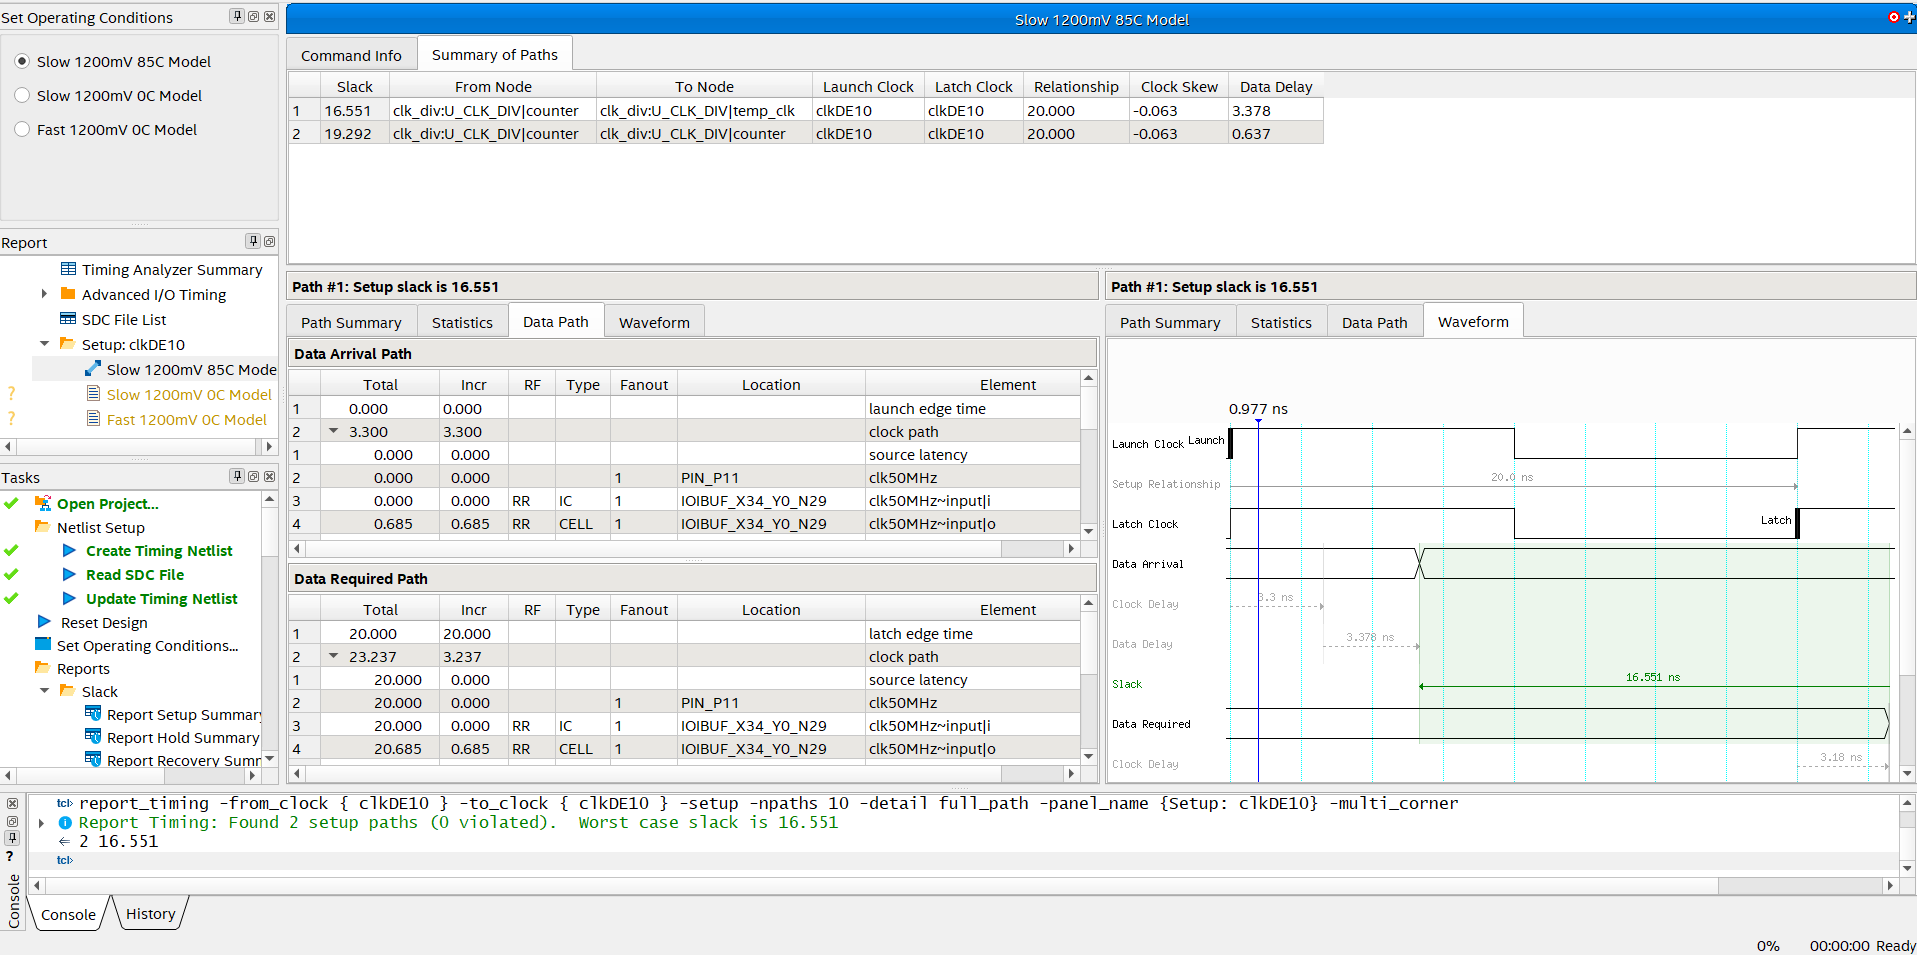
\includegraphics[width=0.8\textwidth]{P4-Report-Timing-20ns.png}
  \caption{VGA Part 3 Timing Analysis}
\end{figure}

\end{document}
